\documentclass[a4paper,11pt]{article}

\usepackage{graphicx}
\usepackage{booktabs}
% \usepackage{lmodern}
\usepackage{newtxtext,newtxmath}

\usepackage{geometry}
\geometry{top=2cm, left=2cm, right=2cm, bottom=2cm}
\pagestyle{empty}

%% define macro
% https://latex.org/forum/viewtopic.php?t=3970
\makeatletter
\newcommand*\ExpandableInput[1]{\@@input#1 }
\makeatother

\begin{document}


%%%%%%%%%%
%%%%%%%%%%
\begin{figure}[htbp]
 \centering
 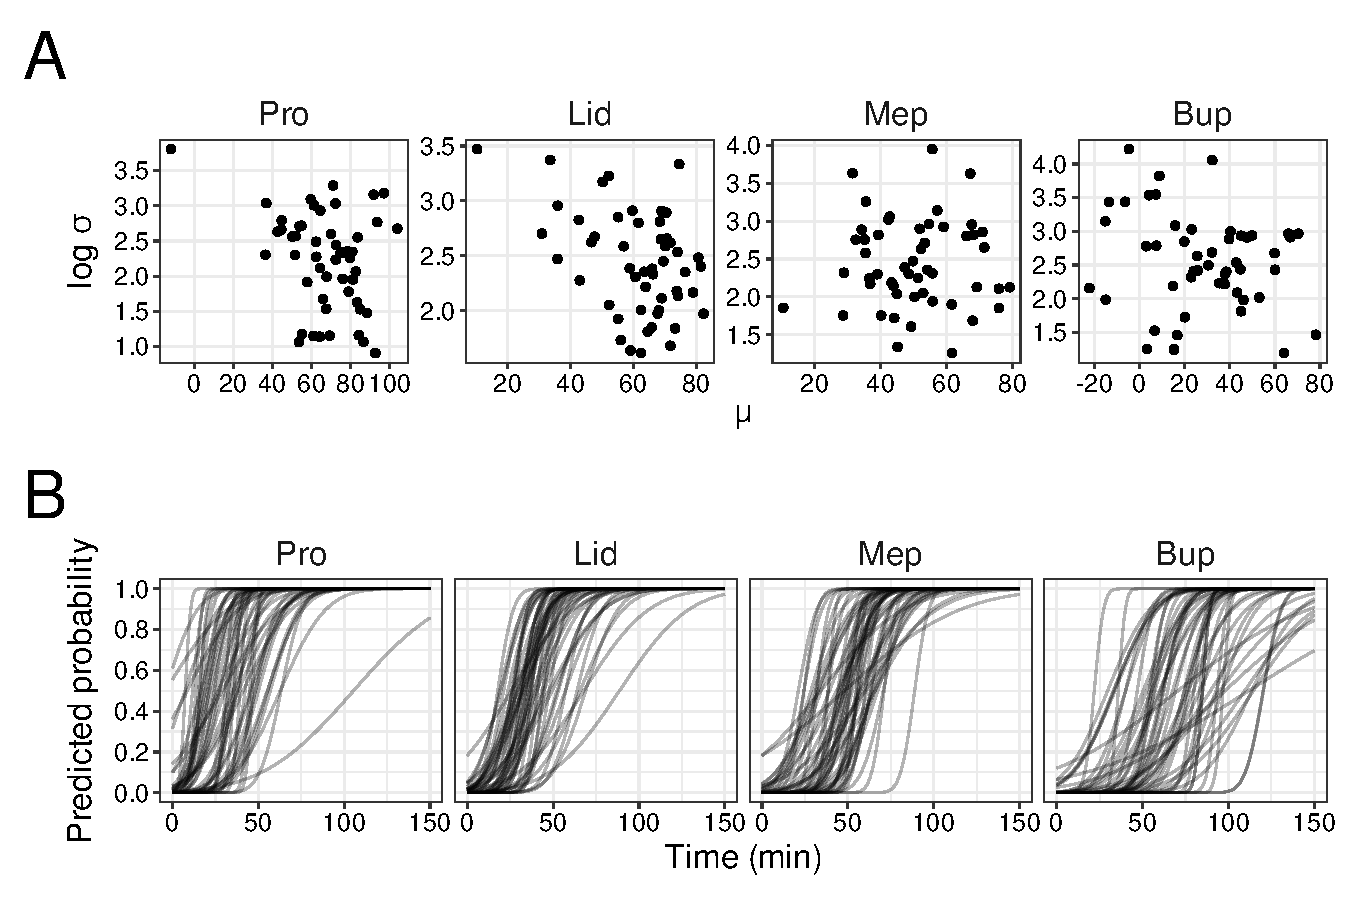
\includegraphics[width=0.9\textwidth]{Fig/Fig1.pdf}
 \caption{Correlation of parameters between $\mu$ and $\log \sigma$
  in animal experiments.
  (A) scatter plot of $\mu$ and $\log \sigma$ in each drug,
  and
  (B) Predicted probability curve in each drug and individual.}
 \label{fig1}
\end{figure}
%%%%%%%%%%
%%%%%%%%%%

\clearpage


%%%%%%%%%%
%%%%%%%%%%
\begin{figure}[htbp]
 \centering
 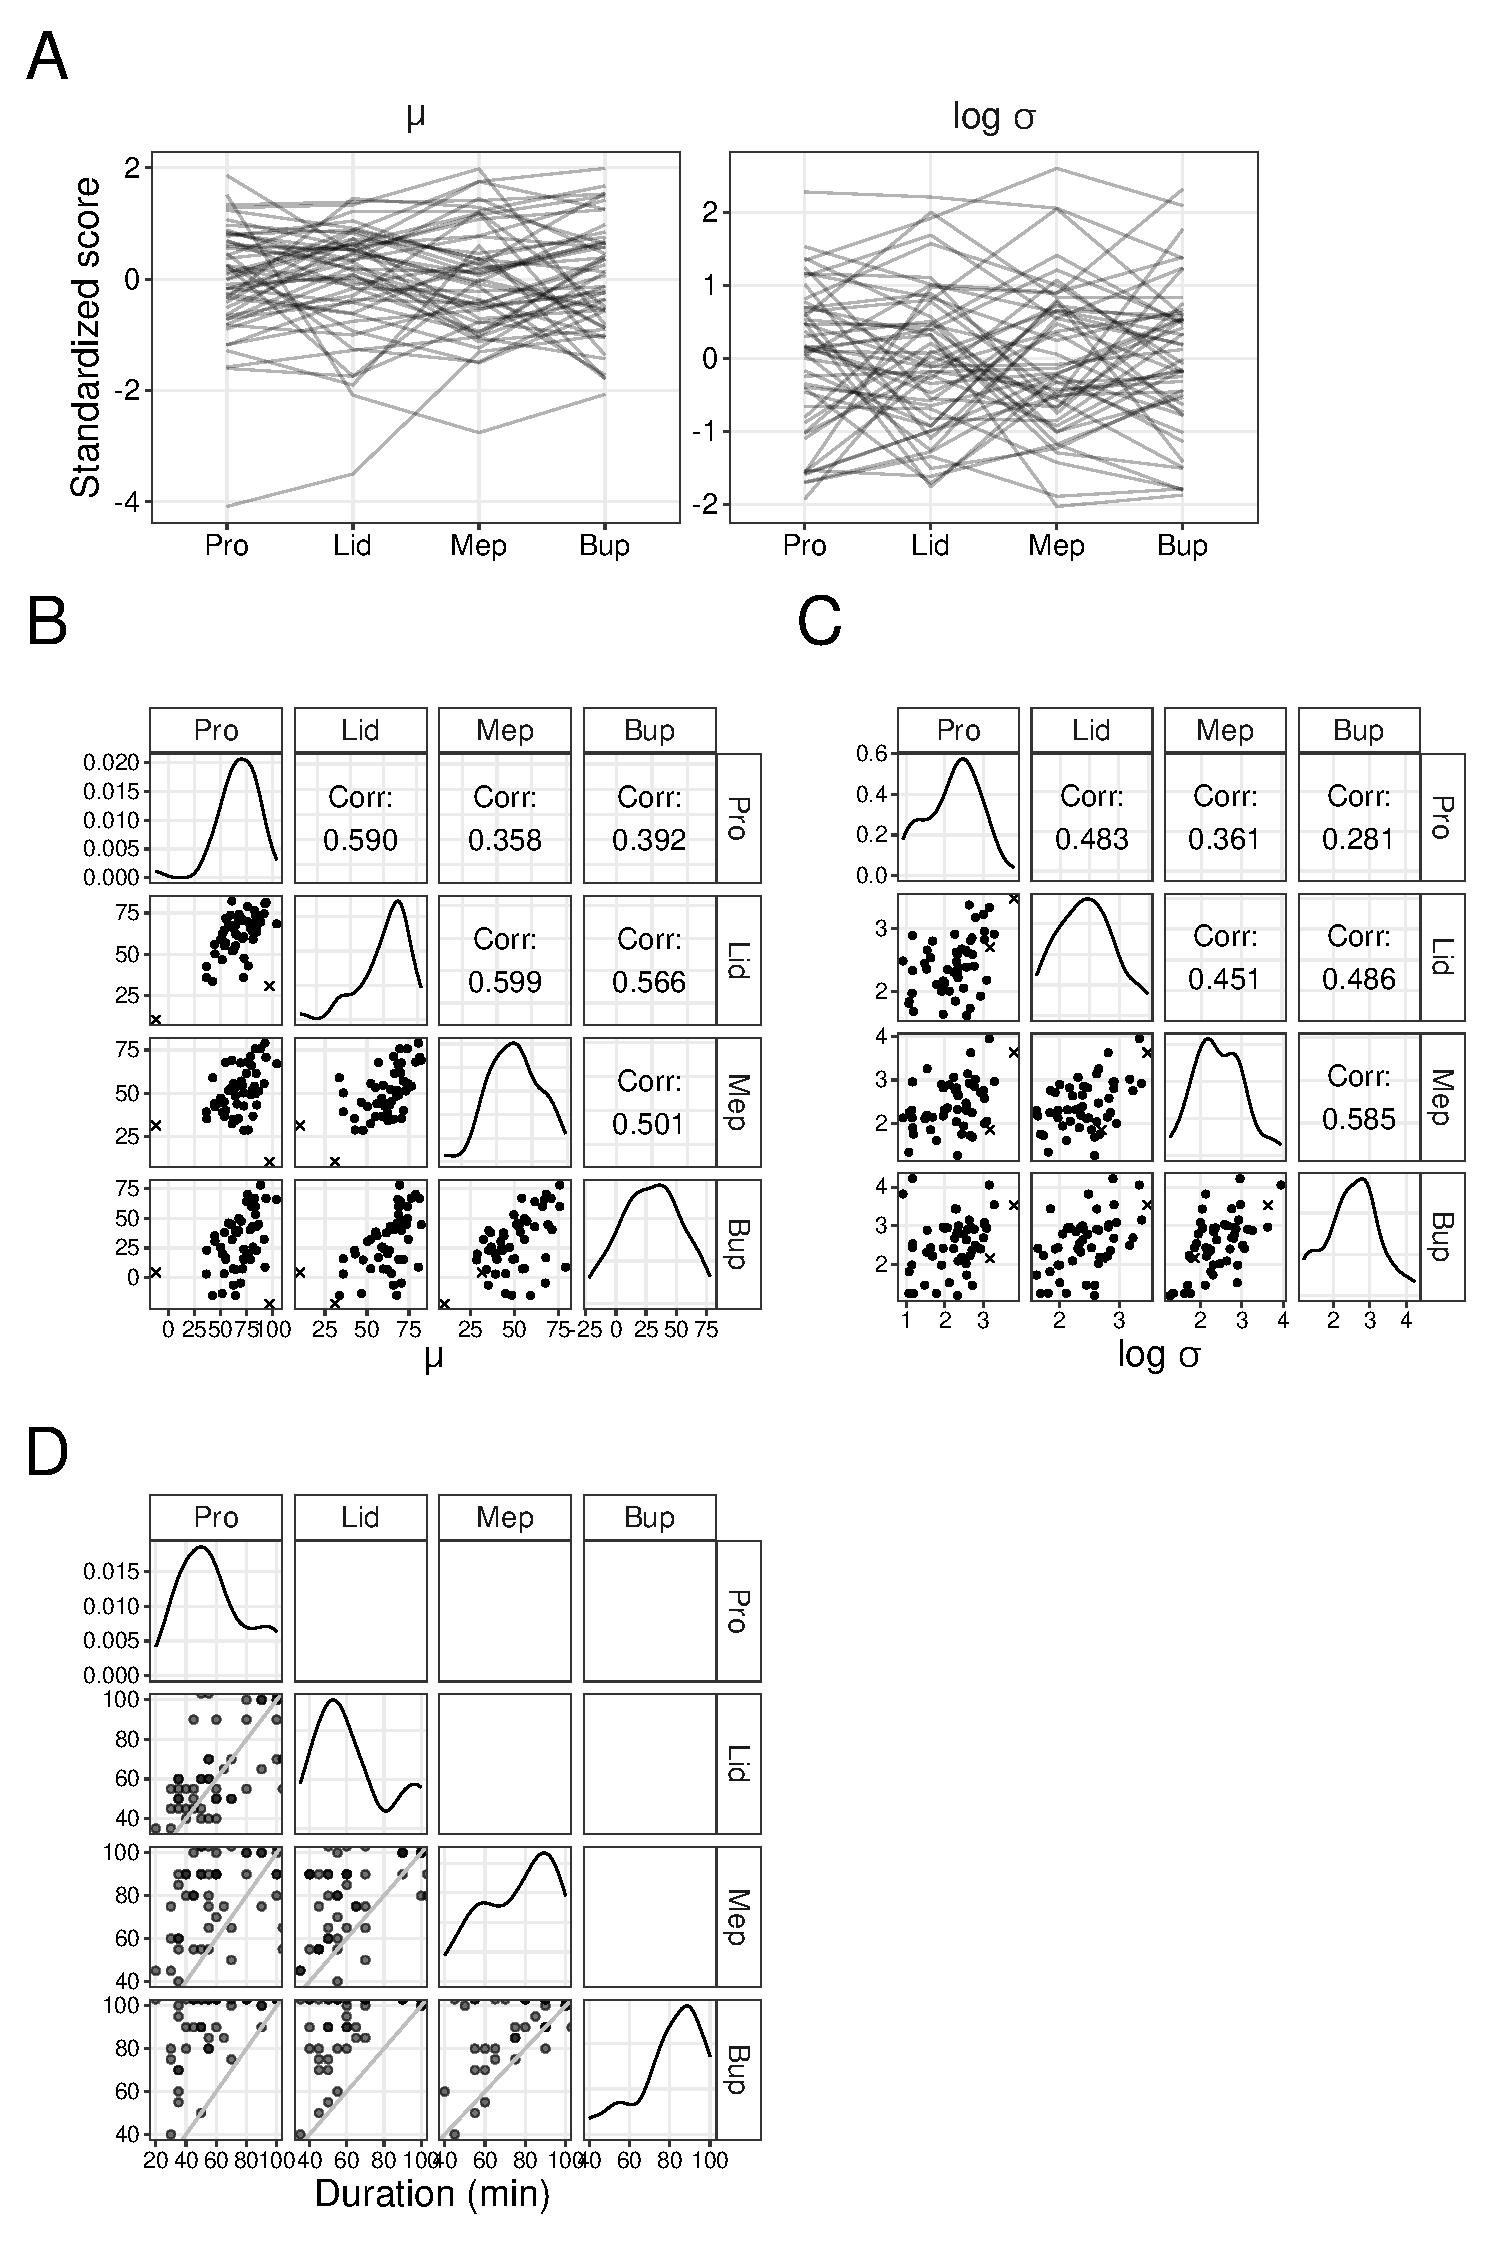
\includegraphics[width=0.8\textwidth]{Fig/Fig2.pdf}
 \caption{Correlation of parameters among drugs in animal experiments.}
 \label{fig2}
\end{figure}
%%%%%%%%%%
%%%%%%%%%%

\clearpage


%%%%%%%%%%
%%%%%%%%%%
\begin{table}[htbp]
 \caption{Correlation coefficients between $\mu$ and $\log \sigma$ ($r_{\mu - \log \sigma}$)}
 \label{tbl1}
 \small
 \vspace{1ex}
 \centering
 \begin{tabular}{ccc}
  \toprule
  \ExpandableInput{Table/Table1.tex}
 \end{tabular}
\end{table}
%%%%%%%%%%
%%%%%%%%%%


%%%%%%%%%%
%%%%%%%%%%
\begin{table}[htbp]
 \caption{Correlation coefficients among drugs}
 \label{tbl2}
 \small
 \vspace{1ex}
 \centering
 \begin{tabular}{ccccc}
  \toprule
   & \multicolumn{2}{c}{all data ($n = 51$)}
   & \multicolumn{2}{c}{without outliers ($n = 49$)} \\
  \cmidrule(lr){2-3}
  \cmidrule(lr){4-5}
  \ExpandableInput{Table/Table2.tex}
 \end{tabular}
\end{table}
%%%%%%%%%%
%%%%%%%%%%



%%%%%%%%%%
%%%%%%%%%%
\begin{table}[htbp]
 \caption{Parameters used in simulations}
 \label{tbl3}
 \small
 \vspace{1ex}
 \centering
 \begin{tabular}{ccccccccc}
  \toprule
  \ExpandableInput{Table/Table3.tex}
 \end{tabular}
\end{table}
%%%%%%%%%%
%%%%%%%%%%

\clearpage



%%%%%%%%%%
%%%%%%%%%%
\begin{figure}[htbp]
 \centering
 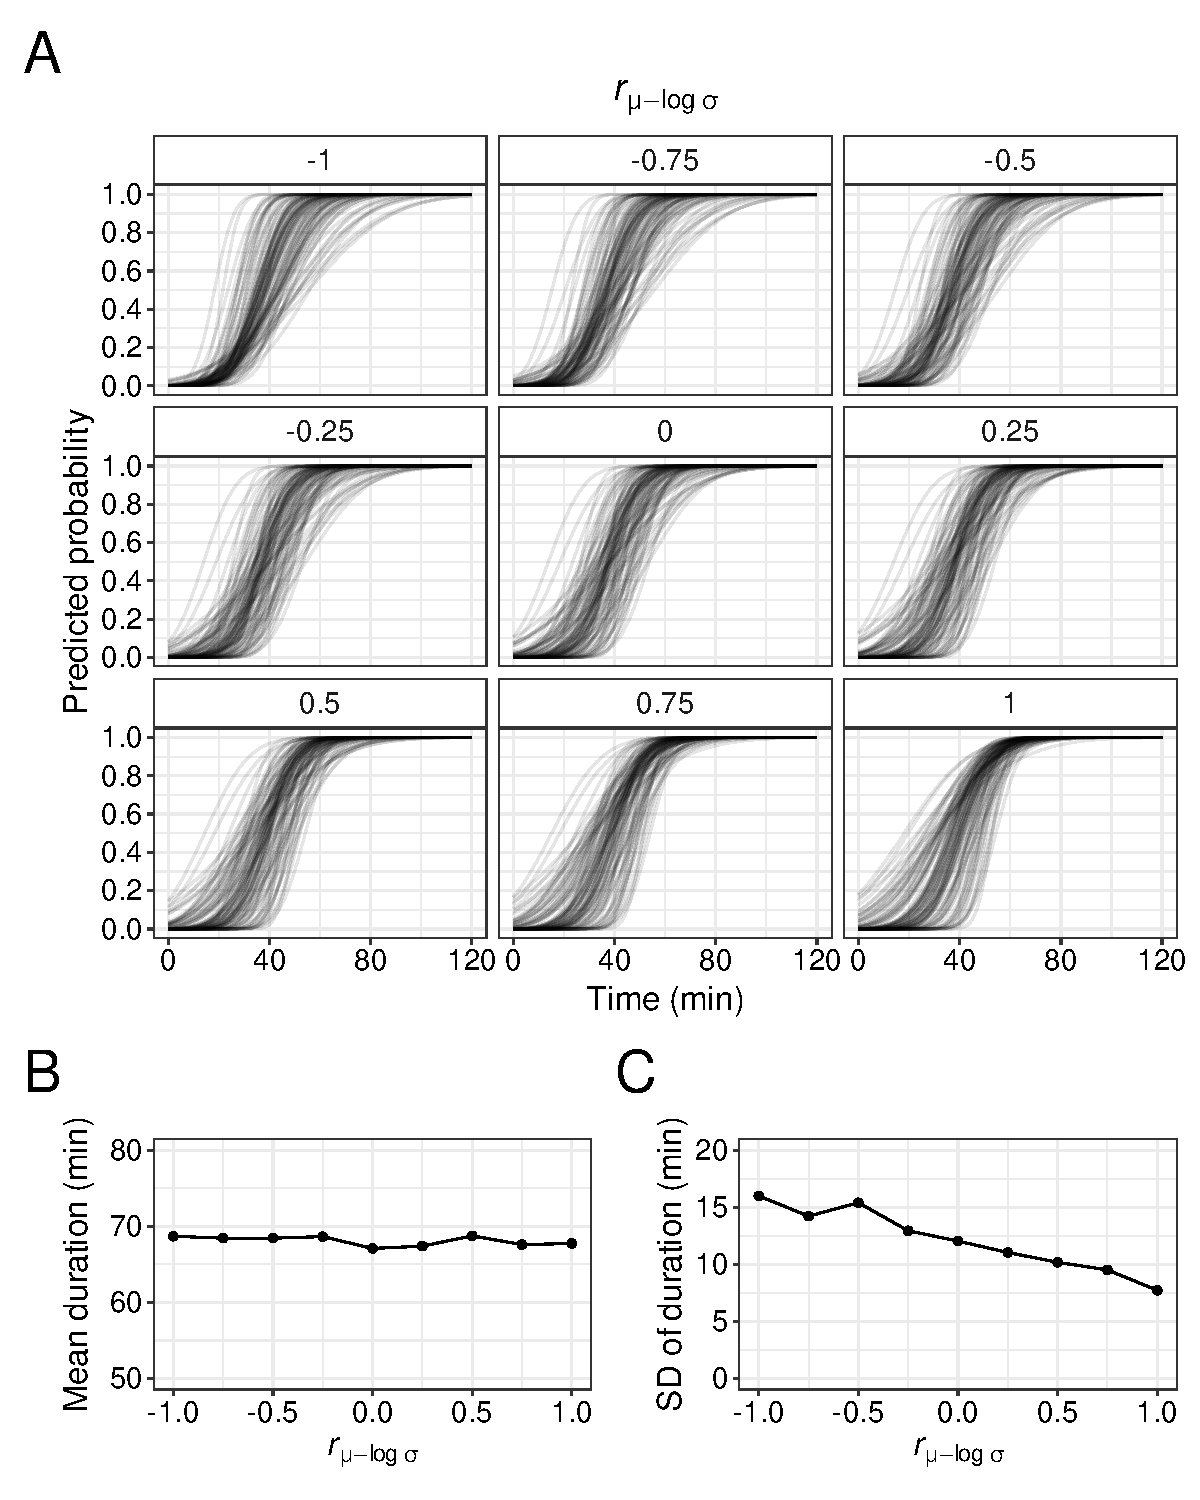
\includegraphics[width=0.8\textwidth]{Fig/Fig3.pdf}
 \caption{Effect of correlation of parameters
           between $\mu$ and $\log \sigma$ ($r_{\mu - \log \sigma}$)
           on duration of Lid in simulation.}
 \label{fig3}
\end{figure}
%%%%%%%%%%
%%%%%%%%%%

\clearpage



%%%%%%%%%%
%%%%%%%%%%
\begin{figure}[htbp]
 \centering
 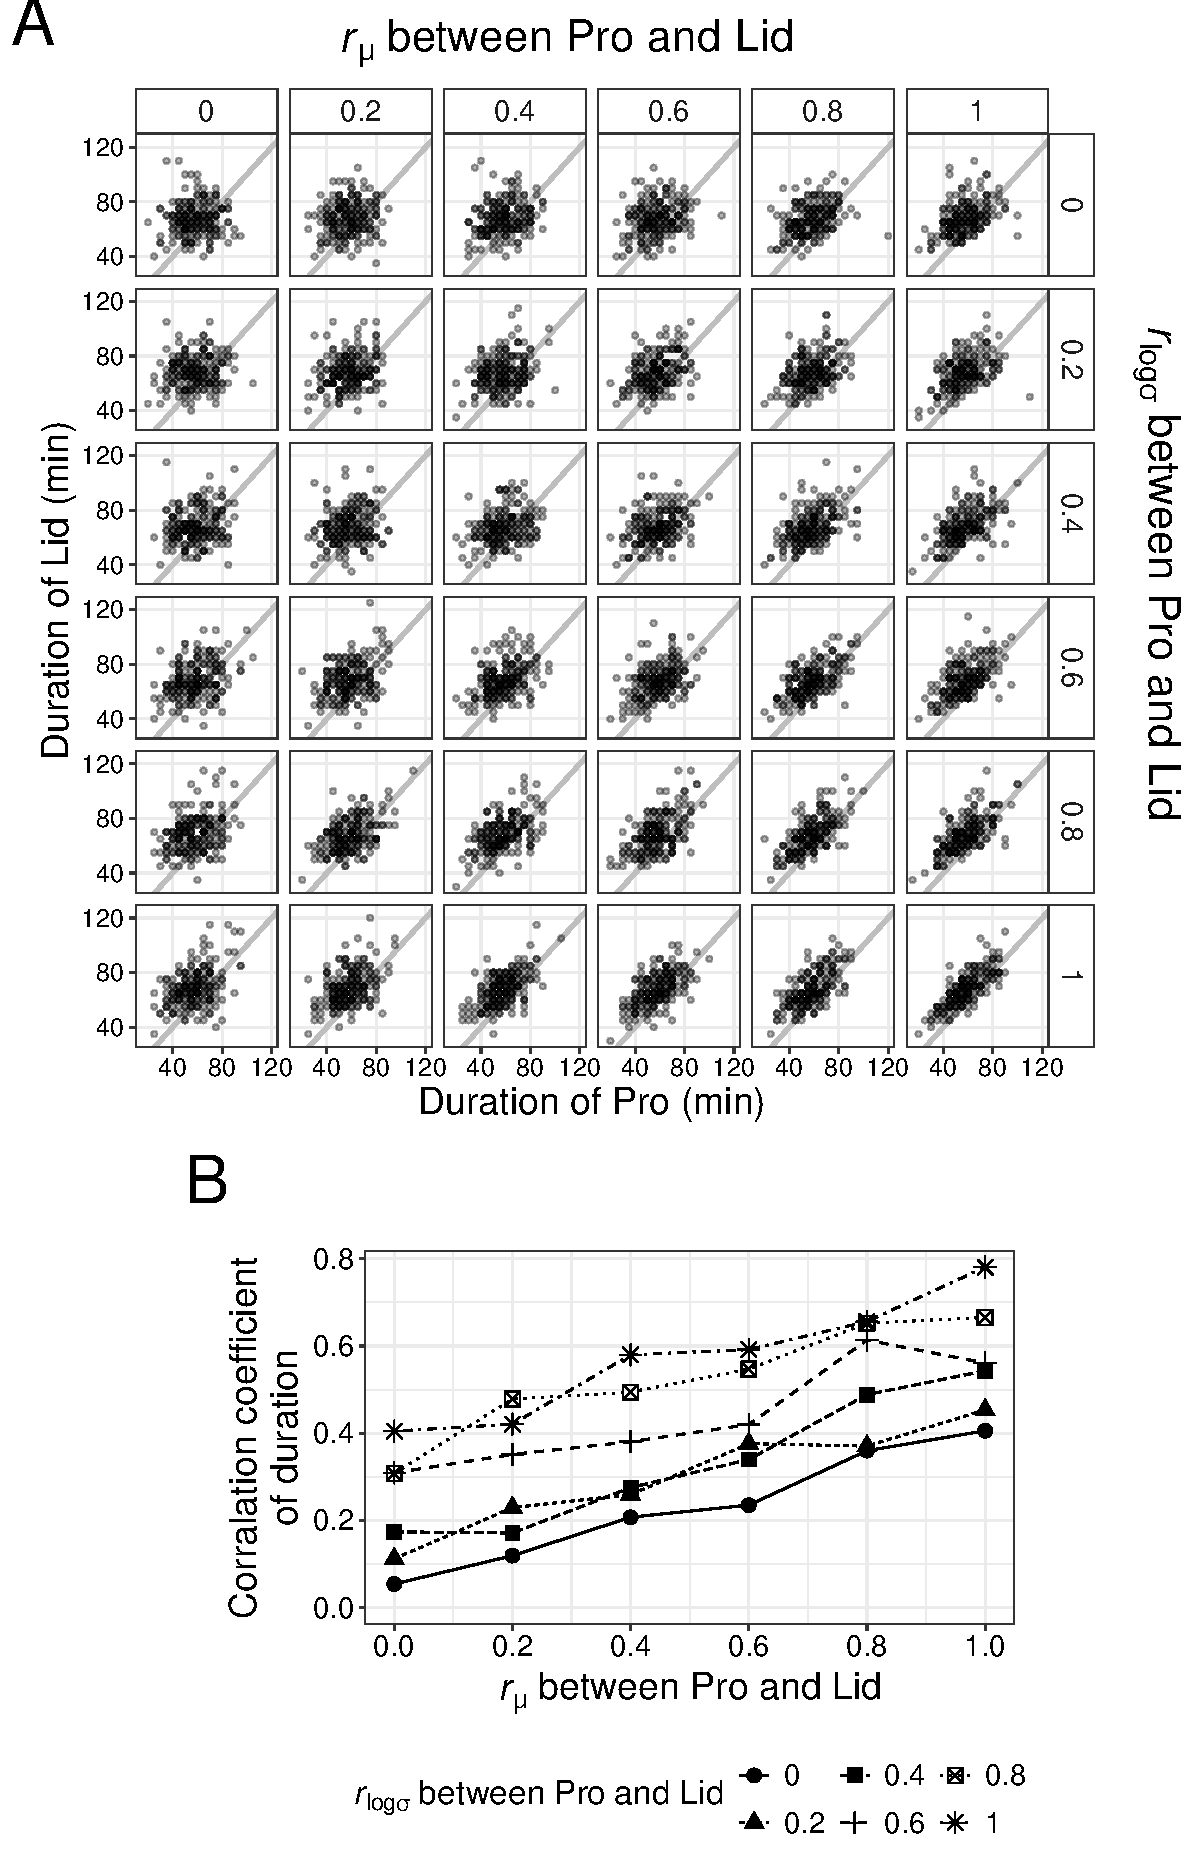
\includegraphics[width=0.8\textwidth]{Fig/Fig4.pdf}
 \caption{Effect of correlation of parameters ($r_{\mu}$ and $r_{\log \sigma}$) between Pro and Lid on duration in simulation ($r_{\mu - \log \sigma}$ is set to 0). (A) Relation of durations between Pro and Lid. (B) Correlation coefficients of duration in several parameters.}
 \label{fig4}
\end{figure}
%%%%%%%%%%
%%%%%%%%%%

\clearpage



%%%%%%%%%%
%%%%%%%%%%
\begin{figure}[htbp]
 \centering
 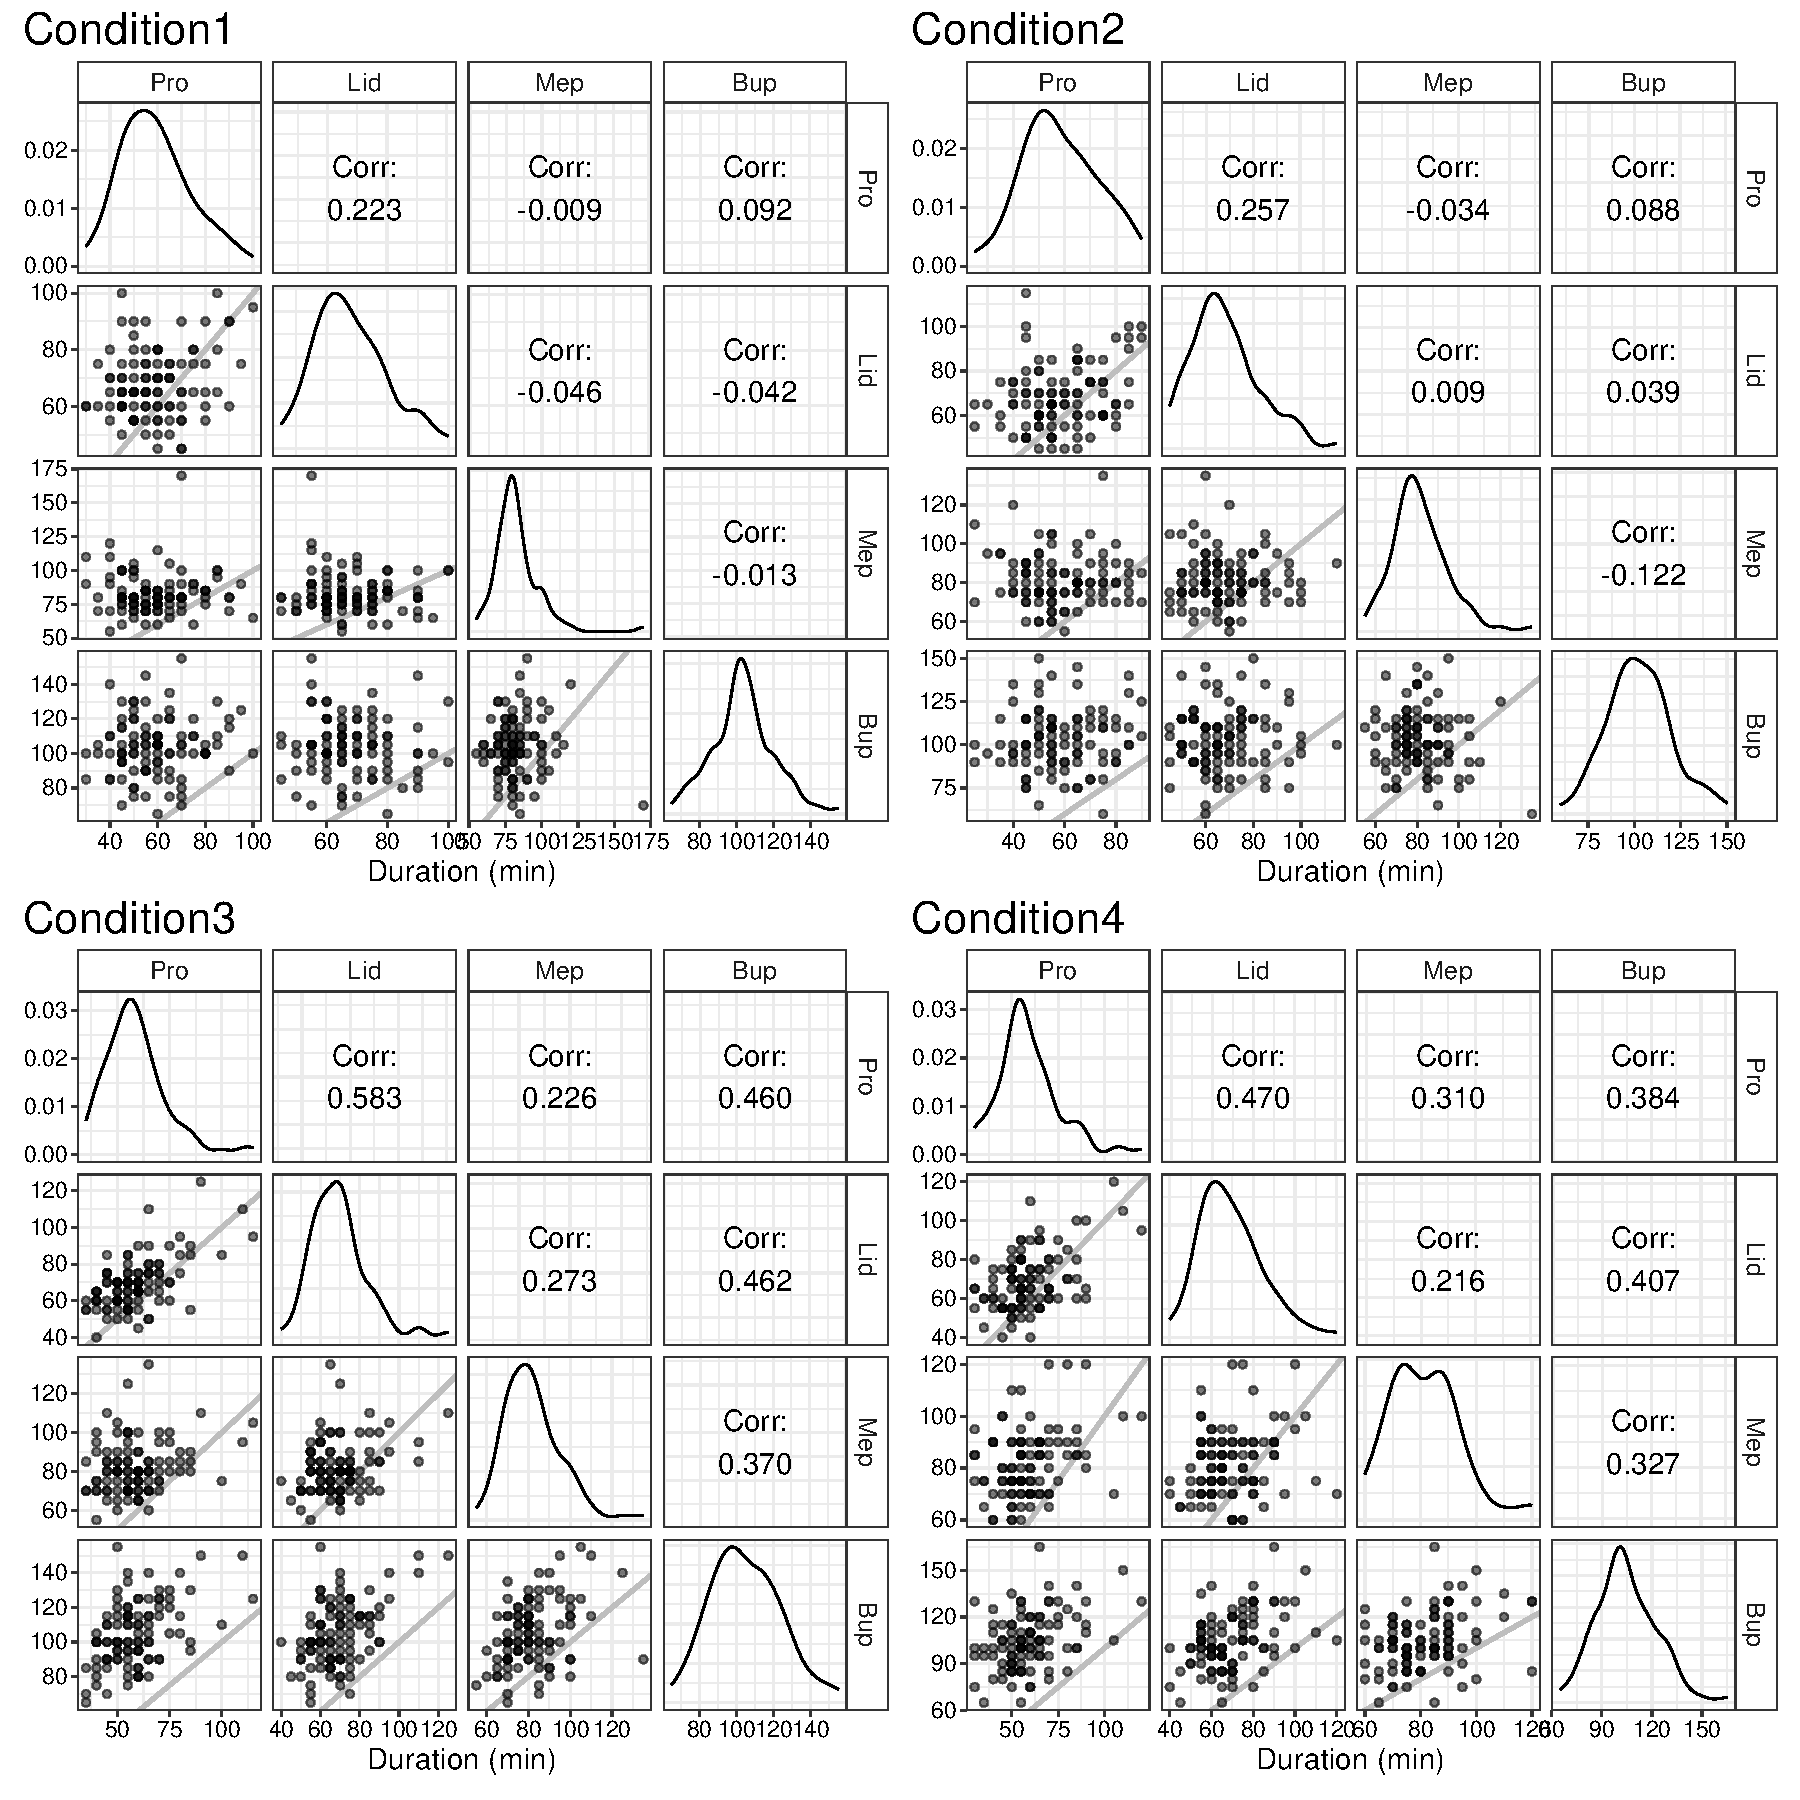
\includegraphics[width=1\textwidth]{Fig/Fig5.pdf}
 \caption{Effect of correlation of parameters among drugs on duration in simulation.}
 \label{fig5}
\end{figure}
%%%%%%%%%%
%%%%%%%%%%

\clearpage



%%%%%%%%%%
%%%%%%%%%%
\begin{table}[htbp]
 \caption{Effect of correlation coefficients on duration among drugs}
 \label{tbl4}
 \small
 \vspace{1ex}
 \centering
 \begin{tabular}{ccccccc}
  \toprule
  & Condition 1 & Condition 2 & Condition 3 & Condition 4 \\
  \midrule
  $r_{\mu - \log \sigma}$         & 0 & * & 0 & * \\
  $r_{\mu}$ and $r_{\log \sigma}$ & 0 & 0 & * & * \\
  \ExpandableInput{Table/Table4.tex}

  \\[-2ex]
  \multicolumn{5}{r}{$^\text{*}$Parameters in Table \ref{tbl3} were used.} \\
 \end{tabular}
\end{table}
%%%%%%%%%%
%%%%%%%%%%



%%%%%%%%%%
%%%%%%%%%%
\begin{table}[htbp]
 \caption{Median of duration of local anesthetic agents under each condition}
 \label{tbl5}
 \small
 \vspace{1ex}
 \centering
 \begin{tabular}{ccccc}
  \toprule
  \ExpandableInput{Table/Table5.tex}
 \end{tabular}
\end{table}
%%%%%%%%%%
%%%%%%%%%%




%%%%%%%%%%
%%%%%%%%%%
\begin{table}[htbp]
 \caption{Comparison of duration between Pro and Lid}
 \label{tbl6}
 \small
 \vspace{1ex}
 \centering
 \begin{tabular}{ccccccc}
  \toprule
  \ExpandableInput{Table/Table6.tex}
 \end{tabular}
\end{table}
%%%%%%%%%%
%%%%%%%%%%

\clearpage



%%%%%%%%%%%%%%%%%%%%%%%%%%%%%%%%%%%%%%%%
%% Supplemental Figure / Table
%%%%%%%%%%%%%%%%%%%%%%%%%%%%%%%%%%%%%%%%

\renewcommand{\figurename}{Supplementary Figure}
\renewcommand{\tablename}{Supplementary Table}
\setcounter{figure}{0}
\setcounter{table}{0}


%%%%%%%%%%
%%%%%%%%%%
\begin{table}[htbp]
 \caption{Spearman's rank correlation coefficients of duration among drugs}
 \label{Stbl1}
 \small
 \vspace{1ex}
 \centering
 \begin{tabular}{ccc}
  \toprule
  \ExpandableInput{Table/STable1.tex}
 \end{tabular}
\end{table}
%%%%%%%%%%
%%%%%%%%%%



% latex table generated in R 4.3.3 by xtable 1.8-4 package
\begin{table}[ht]
\centering
\caption{Analysis by Linear Mixed-Effects Models with interaction} 
\label{Stbl_lmer1}
\begingroup\small
\begin{tabular}{lllrrrrr}
  \toprule
effect & group & term & estimate & std.error & statistic & df & p.value \\ 
  \midrule
fixed &  & (Intercept) & 0.083 & 0.014 & 5.841 & 12.4 & 0.000 \\ 
  fixed &  & r\_mean & 0.398 & 0.012 & 31.931 & 277.0 & 0.000 \\ 
  fixed &  & r\_logSigma & 0.267 & 0.012 & 21.445 & 277.0 & 0.000 \\ 
  fixed &  & r\_mean:r\_logSigma & 0.020 & 0.021 & 0.973 & 277.0 & 0.331 \\ 
  ran\_pars & seed\_param & sd\_\_(Intercept) & 0.034 &  &  &  &  \\ 
  ran\_pars & Residual & sd\_\_Observation & 0.041 &  &  &  &  \\ 
   \bottomrule
\end{tabular}
\endgroup
\end{table}

% % latex table generated in R 4.3.3 by xtable 1.8-4 package
\begin{table}[ht]
\centering
\caption{Analysis by Linear Mixed-Effects Models with interaction} 
\label{Stbl_lmer1}
\begingroup\small
\begin{tabular}{lllrrrrr}
  \toprule
effect & group & term & estimate & std.error & statistic & df & p.value \\ 
  \midrule
fixed &  & (Intercept) & 0.083 & 0.014 & 5.841 & 12.4 & 0.000 \\ 
  fixed &  & r\_mean & 0.398 & 0.012 & 31.931 & 277.0 & 0.000 \\ 
  fixed &  & r\_logSigma & 0.267 & 0.012 & 21.445 & 277.0 & 0.000 \\ 
  fixed &  & r\_mean:r\_logSigma & 0.020 & 0.021 & 0.973 & 277.0 & 0.331 \\ 
  ran\_pars & seed\_param & sd\_\_(Intercept) & 0.034 &  &  &  &  \\ 
  ran\_pars & Residual & sd\_\_Observation & 0.041 &  &  &  &  \\ 
   \bottomrule
\end{tabular}
\endgroup
\end{table}

% % latex table generated in R 4.3.3 by xtable 1.8-4 package
\begin{table}[ht]
\centering
\caption{Analysis by Linear Mixed-Effects Models without interaction} 
\label{Stbl_lmer2}
\begin{tabular}{lllrrrrr}
  \toprule
effect & group & term & estimate & std.error & statistic & df & p.value \\ 
  \midrule
fixed &  & (Intercept) & 0.078 & 0.013 & 5.885 & 9.4 & 0.000 \\ 
  fixed &  & r\_mean & 0.408 & 0.007 & 58.038 & 278.0 & 0.000 \\ 
  fixed &  & r\_logSigma & 0.277 & 0.007 & 39.447 & 278.0 & 0.000 \\ 
  ran\_pars & seed\_param & sd\_\_(Intercept) & 0.034 &  &  &  &  \\ 
  ran\_pars & Residual & sd\_\_Observation & 0.041 &  &  &  &  \\ 
   \bottomrule
\end{tabular}
\end{table}

% % latex table generated in R 4.3.3 by xtable 1.8-4 package
\begin{table}[ht]
\centering
\caption{Likelihood ratio test of two models} 
\label{Stbl_lmer_LRtest}
\begin{tabular}{lrrrrrrrr}
  \toprule
term & npar & AIC & BIC & logLik & deviance & statistic & df & p.value \\ 
  \midrule
lmer2 & 5 & -993.2 & -974.9 & 501.6 & -1003.2 &  &  &  \\ 
  lmer1 & 6 & -992.1 & -970.1 & 502.1 & -1004.1 & 0.956 & 1 & 0.328 \\ 
   \bottomrule
\end{tabular}
\end{table}




%%%%%%%%%%
%%%%%%%%%%
\begin{table}[htbp]
 \caption{Effect of Spearman's rank correlation coefficients on duration among drugs}
 \label{Stbl3}
 \small
 \vspace{1ex}
 \centering
 \begin{tabular}{ccccccc}
  \toprule
  & Condition 1 & Condition 2 & Condition 3 & Condition 4 \\
  \midrule
  $r_{\mu - \log \sigma}$         & 0 & * & 0 & * \\
  $r_{\mu}$ and $r_{\log \sigma}$ & 0 & 0 & * & * \\
  \ExpandableInput{Table/STable3.tex}

  \\[-2ex]
  \multicolumn{5}{r}{$^\text{*}$Parameters in Table \ref{tbl3} were used.} \\
 \end{tabular}
\end{table}
%%%%%%%%%%
%%%%%%%%%%

\end{document}

